\documentclass[11pt]{article}
\usepackage[a4paper,margin=26mm]{geometry}
\usepackage[T1]{fontenc}
\usepackage{lmodern}
\usepackage{amsmath,amssymb,amsthm}
\usepackage{microtype}
\usepackage{array}
\usepackage{tikz}
\usepackage{wrapfig}
\usepackage{xurl}
\usepackage{hyperref}
\hypersetup{colorlinks=true,linkcolor=blue,urlcolor=blue,citecolor=blue,
 pdftitle={The discrete quantitative Helly number for five common lattice points},
 pdfauthor={Horace Dong}}
\newtheorem{theorem}{Theorem}
\newtheorem{lemma}{Lemma}
\newtheorem{proposition}{Proposition}
\newtheorem{corollary}{Corollary}
\theoremstyle{definition}
\newtheorem{definition}{Definition}
\theoremstyle{remark}
\newtheorem{remark}{Remark}
\newcommand{\repoversion}{1.26.0}
\setlength{\emergencystretch}{1.5em}
\newcommand{\Z}{\mathbb Z}
\newcommand{\R}{\mathbb R}
\newcommand{\vertx}{\operatorname{vert}}
\newcommand{\conv}{\operatorname{conv}}

\title{The discrete quantitative Helly number\\ for five common lattice points}
\author{Horace Dong\\ \small Independent researcher\\
\small\texttt{maxwelldhx@gmail.com}\\
\small ORCID: \href{https://orcid.org/0009-0002-7554-7548}{0009-0002-7554-7548}}
\date{23 November 2026}
\begin{document}
\sloppy
\maketitle

\begin{abstract}
For a set $S\subseteq\R^n$ and $k\ge0$, the discrete quantitative Helly
number $c(S,k)$ of Averkov, Gonz\'alez Merino, Paschke, Schymura and Weltge is
the least $t$ such that whenever finitely many convex sets have exactly $k$
points of $S$ in common, at most $t$ of them already have exactly the same $k$
points of $S$ in common. For $n\ge2$ the values for $k\le4$ are known
(collected in their Theorem~5; the cases $k=1$ and $k=2$ are due to Aliev et
al.\ and to Chestnut, Hildebrand and Zenklusen), and Averkov et al.\ computed
the values for $n=2$ and all $k\le30$. We determine the next case: for
$n=1,2,3$ we have $c(\Z^n,5)=2,7,18$, and for every $n\ge4$
\[
c(\Z^n,5)=2^{n+1}+5 .
\]
The value for $n=2$ was known, and the case $n=1$ is elementary. The same numbers are the largest numbers of
vertices of a lattice polytope in $\R^n$ with exactly five lattice points that
are not vertices. The upper bound comes from a parity argument: three lattice
points of a polytope in the same class modulo~$2$ are determined by their three
pairwise midpoints, which are non-vertex lattice points; for $n=3$ a finite
table is added, and for $n=2$ a table and a short planar argument. The lower bound comes from
explicit polytopes with $18$ and $37$ vertices in dimensions $3$ and $4$ and a
lifting construction for $n\ge5$. Both statements are formally verified in
Lean~4. The proofs were found and formalized by AI agents working under the
author's direction; their role is described at the end of the paper.
\end{abstract}

\section{Introduction}\label{sec:intro}

Helly's theorem says that if every $n+1$ members of a finite family of convex
sets in $\R^n$ have a common point, then the whole family has a common point.
Doignon~\cite{doi} proved a lattice version, later rediscovered independently
by Bell, by Scarf and by Hoffman (as reported in~\cite{agm}): if convex sets $C_1,\dots,C_m\subseteq\R^n$
have no point of $\Z^n$ in common, then some $2^n$ of them already have no
point of $\Z^n$ in common, and $2^n$ cannot be replaced by a smaller number.
Aliev, Bassett, De Loera and Louveaux~\cite{abdl} asked the quantitative
question: if a system of linear inequalities has exactly $k$ integer
solutions, how many of the inequalities are needed to keep exactly these
solutions? Averkov, Gonz\'alez Merino, Paschke, Schymura and
Weltge~\cite{agm} gave the following general form.

\begin{definition}[{\cite[Definition~1]{agm}}]\label{def:c}
Let $S\subseteq\R^n$ and $k\in\{0,1,2,\dots\}$. The quantitative Helly number
$c(S,k)$ is the smallest $t\ge0$ such that: if convex sets $C_1,\dots,C_m$
($m\ge1$) have exactly $k$ points of $S$ in common, then there is a subset $I$
of $\{1,\dots,m\}$ with at most $t$ elements such that the sets $C_i$ with
$i\in I$ already have exactly $k$ points of $S$ in common (with
$c(S,k)=\infty$ if no such $t$ exists).
\end{definition}

\noindent The sets are arbitrary convex sets (not necessarily closed or
bounded), and the empty subfamily is allowed (its common points are all of
$S$). Throughout we cite~\cite{agm} by the numbering of arXiv:1602.07839v1,
the only arXiv version, whose author list has M.~Henze in place of
M.~Schymura. According to the notes of the Codex agents, some section and lemma
numbers differ in the journal version, which we could not read.

\paragraph{The polytope description.}
A \emph{lattice polytope} is the convex hull of finitely many points of $\Z^n$
(of any dimension). For such a polytope $P$, a lattice point of $P$ is either a
vertex of $P$ or a \emph{non-vertex lattice point} of $P$; the latter may lie
in the interior or on the boundary. Averkov et al.\ introduced
\[
g(S,k)=\max\{|\vertx(P)| : P\in\mathcal P(S),\ |S\cap P\setminus\vertx(P)|=k\},
\]
where $\mathcal P(S)$ is the set of polytopes with vertices in $S$, and proved
that for discrete $S$ the values $g(S,k)$ determine the values $c(S,k)$ through
the recursion~\cite[Theorem~2,~(5)]{agm}
\begin{equation}\label{eq:rec}
c(S,0)=g(S,0),\qquad c(S,k)=\max\{c(S,k-1)-1,\ g(S,k)\}\quad (0<k\le|S|).
\end{equation}
An equivalent form is $c(S,k)=\max\{|S\cap P|-k\}$ over the polytopes
$P\in\mathcal P(S)$ with $|S\cap P\setminus\vertx(P)|\le k\le|S\cap P|$
\cite[(6)]{agm}. So the Helly-type question about arbitrary convex sets
becomes a question about lattice polytopes with few non-vertex lattice points.

\paragraph{Known values.}
Doignon's theorem is $c(\Z^n,0)=2^n$. For $n\ge2$, Theorem~5
of~\cite{agm} collects the values
\[
c(\Z^n,1)=c(\Z^n,2)=c(\Z^n,3)=2^{n+1}-2,\qquad c(\Z^n,4)=2^{n+1};
\]
the case $k=1$ is due to Aliev et al.~\cite[Theorem~2]{abdl}, the case $k=2$ to
Chestnut et al.~\cite[Proposition~4.5]{chz}, and the cases $k=3,4$ to Averkov
et al. Averkov et al.\ also, from Castryck's database of lattice polygons, they computed
$g(\Z^2,k)=c(\Z^2,k)$ for all $k\le30$ \cite[Figure~3]{agm}. In particular
$c(\Z^2,5)=7<8=c(\Z^2,4)$; this value was also proved by Chestnut,
Hildebrand and Zenklusen~\cite[Section~5, Lemma~5.2 and Figure~1]{chz}, who also showed
that $|c(n,k)-2^{n+1}|=O(1)$ for every fixed $k\ge1$
\cite[Corollary~3.13]{chz}, for their version $c(n,k)$ of the number (defined
through rows of a system $Ax\le b$). For $n=1$, every lattice polytope is a
point or a segment, so $g(\Z,k)=2$ for all $k\ge0$, and~\eqref{eq:rec} gives
$c(\Z,k)=2$ for all $k$.

\paragraph{The result.} Let
\[
v(1)=2,\qquad v(2)=7,\qquad v(3)=18,\qquad v(n)=2^{n+1}+5\quad(n\ge4),
\]
so that $v(4)=37$, $v(5)=69$ and $v(6)=133$.

\begin{theorem}\label{thm:main}
For every $n\ge1$,
\[
c(\Z^n,5)=g(\Z^n,5)=v(n).
\]
That is, (i) if convex sets in $\R^n$ have exactly five lattice points in
common, then at most $v(n)$ of them already have exactly these five lattice points
in common, and $v(n)$ cannot be replaced by a smaller number; and (ii) every
lattice polytope in $\R^n$ with exactly five non-vertex lattice points has at
most $v(n)$ vertices, and there is one with exactly $v(n)$ vertices.
\end{theorem}

Both parts are formally verified in Lean~4 (Section~\ref{sec:lean}); Lean
proves the value of $c(\Z^n,5)$ directly from Definition~\ref{def:c}, not
through~\eqref{eq:rec}. The two parts are also consistent through~\eqref{eq:rec}:
since $c(\Z^n,4)=2^{n+1}$ for $n\ge2$, the recursion gives
$c(\Z^n,5)=g(\Z^n,5)$ exactly when $g(\Z^n,5)\ge c(\Z^n,4)-1=2^{n+1}-1$, and
this holds ($7\ge7$, $18\ge15$, and $2^{n+1}+5\ge2^{n+1}-1$). The main
step of the upper bound is the following statement, which is also proved in
Lean (as \texttt{Proof.poly\_bound}).

\begin{theorem}\label{thm:poly}
Let $P$ be a lattice polytope in $\R^n$ with at most five non-vertex lattice
points. Then $P$ contains at most $v(n)+5$ lattice points, that is, at most
$7$, $12$, $23$ or $2^{n+1}+10$ lattice points for $n=1$, $n=2$, $n=3$ or
$n\ge4$, respectively.
\end{theorem}

\paragraph{Scope.}
The result is for Definition~\ref{def:c}, with finite families of arbitrary
convex sets. The original number $c(n,k)$ of Aliev et al.~\cite[Theorem~1]{abdl}
is defined through subsets of the rows of a system $Ax\le b$ (their abstract
speaks of a bounded polyhedron, their Theorem~1 of an arbitrary polyhedron
$\{x:Ax\le b\}$). Definition~\ref{def:c} is linked to it through Lemma~8
of~\cite{agm} (closed halfspaces suffice) and considerations about
boundedness; this link is not formalized, and we make no separate claim about
that variant. Theorem~\ref{thm:main} also shows $c(\Z^n,5)=g(\Z^n,5)$ for every
$n$. Averkov et al.\ asked whether $c(\Z^n,k)>g(\Z^n,k)$ can happen for some
$n$ and $k$~\cite[Open question~3]{agm}; our result adds the case $k=5$ in every
dimension (for $n=2$ it was known) to the cases $k\le4$ in which equality is
known, but it does not answer the
question. Their other two open questions are not addressed either.

\paragraph{Prior work and what is new.}
The definition, the polytope description~\eqref{eq:rec}, the values for
$k=3,4$ and the planar values are due to~\cite{agm} (the cases $k=1,2$
to~\cite{abdl,chz}); the planar value $c(\Z^2,5)=7$
also to~\cite{chz}. Sorting lattice points into classes modulo~$2$ and using
their midpoints, which are again lattice points, is a method used throughout
the work of Chestnut, Hildebrand and Zenklusen~\cite[Sections~1 and~3]{chz};
Averkov et al.\ use it in their proof of $c(\Z^n,4)=2^{n+1}$
\cite[Section~5]{agm}, including the fact that a triangle is determined by its
edge midpoints (Lemma~\ref{lem:triple}), which they use to charge each class
with three vertices to a facet of $\conv(X)$; and Chestnut et al.\ sort all lattice points of a
planar polytope by parity in their proof of $c(\Z^2,5)\le7$
\cite[Lemma~5.2]{chz}. Proposition~\ref{prop:charge} extends that charging step from the facets of a
tetrahedron to all $3$-subsets of $X$; this general form was not found by the
searches, but it is an elementary step of this method, and we do not claim the
method as new. What we add is its application to $k=5$, together with the
matching constructions and the Lean proof.
Huicochea and Navarro~\cite{hn} improved the lower bounds of~\cite{chz} on
the number of midpoints of vertex pairs of convex polytopes and applied them to
a quantitative Helly-type theorem. Their Helly number is the least $c$ such that,
whenever every $c$ members of a finite family of convex sets have at least
$k+1$ common lattice points, the whole family has; this differs from
Definition~\ref{def:c}. They give an explicit upper bound that grows
sublinearly in $k$ \cite[Theorem~1.8]{hn}; their paper contains no exact values,
and our result is not an improvement of theirs. What is new here, as far as the
searches described at the end found, is the value $18$ for $n=3$, the
formula $2^{n+1}+5$ for $n\ge4$ (the value $37$ for $n=4$ included), and the
polytopes that attain them.

\section{From convex sets to lattice polytopes}\label{sec:reduction}

We use only the two implications of the polytope description that are needed
for $k=5$. They are special cases of~\cite[Theorem~2 and~(6)]{agm}; the Lean
files prove them directly.

\begin{proposition}\label{prop:transfer}
Let $n\ge1$ and $b\ge0$.
\begin{enumerate}
\item[(a)] If a lattice polytope $P\subseteq\R^n$ has $t$ vertices and exactly
five non-vertex lattice points, then $c(\Z^n,5)\ge t$.
\item[(b)] If every lattice polytope in $\R^n$ with at most five non-vertex
lattice points contains at most $b+5$ lattice points, then $c(\Z^n,5)\le b$
and $g(\Z^n,5)\le b$.
\end{enumerate}
\end{proposition}

\begin{proof}
(a) Let $p_1,\dots,p_t$ be the vertices of $P$ and $C_i=P\setminus\{p_i\}$.
Removing an extreme point from a convex set leaves a convex set, so each $C_i$
is convex. The lattice points common to all $C_i$ are the lattice points of $P$
other than the vertices: exactly five. If a subfamily omits $C_i$, then $p_i$
lies in all its members, so the subfamily has at least six common lattice
points. Hence every admissible number in Definition~\ref{def:c} is at least
$t$.

(b) The bound for $g$ is immediate: a polytope with $t$ vertices and exactly
five non-vertex lattice points has $t+5$ lattice points. For $c$, let
$C_1,\dots,C_m$ be convex with exactly five common lattice points, forming a
set $X$, and let $I$ be a smallest set of indices whose sets still have exactly
$X$ as common lattice points. By minimality, for each $i\in I$ there is a
lattice point $w_i\notin X$ lying in every $C_j$ with $j\in I$, $j\ne i$. Let
$B$ be the finite set of lattice points of $\conv(X\cup\{w_i\})$ and replace
each $C_i$ by its trace $C_i\cap B$; these traces are convex relative to $B$
(each contains every point of $B$ in its convex hull) and have $X$ as common
part. Enlarge the traces inside $B$ as far as possible, keeping these
properties. In the enlarged system every index $i\in I$ has a \emph{contact
point} $w'_i\in B$: it lies outside the $i$-th trace, inside all the others
(by maximality: otherwise adding $w'_i$ to the $i$-th trace would keep the
common part $X$), and it is a vertex of the convex hull of the $i$-th trace
together with $w'_i$. The contact points are distinct and not in $X$. Since
$P'=\conv(X\cup\{w'_j:j\in I\})$ lies in $\conv(\text{$i$-th trace}\cup\{w'_i\})$
for every $i$, the lattice points of $P'$ are exactly $X$ and the contact
points, and every contact point is a vertex of $P'$. So $P'$ is a lattice polytope with
$|I|+5$ lattice points, and its non-vertex lattice points lie in $X$. By
hypothesis $|I|+5\le b+5$, so $|I|\le b$.
\end{proof}

\noindent The Lean names of all steps are listed in Table~\ref{tab:lean}; the
hypothesis of~(b) is the Lean predicate \texttt{UpperTransfer.PolyBound n b}. So Theorem~\ref{thm:main}
follows from Theorem~\ref{thm:poly} (with $b=v(n)$) and from polytopes with
$v(n)$ vertices and exactly five non-vertex lattice points
(Section~\ref{sec:lower}).


\section{The upper bound: parity classes and midpoint triples}\label{sec:upper}

Let $P$ be a lattice polytope in $\R^n$, let $S=P\cap\Z^n$ be the set of all its
lattice points and $X\subseteq S$ the set of its non-vertex lattice points.
Every $z\in\Z^n$ has a \emph{class} $z\bmod2\in(\Z/2)^n$; there are $2^n$
classes, and we write $S_r$ for the points of $S$ in class $r$.

\begin{lemma}[midpoints]\label{lem:mid}
If $a\ne b$ are points of $S$ in the same class, then $(a+b)/2$ is a lattice
point and lies in $X$.
\end{lemma}

\begin{proof}
$a+b\equiv2a\equiv0\pmod2$, so $(a+b)/2\in\Z^n$; it lies in $P$ by convexity,
and it is the midpoint of a segment in $P$, so it is not a vertex.
\end{proof}

\begin{lemma}[three midpoints determine the triple; cf.~{\cite[proof of Theorem~5]{agm}}]\label{lem:triple}
Let $a,b,c$ be three distinct points of $\Z^n$ in the same class, and let
$u_{ab}=(a+b)/2$, $u_{ac}=(a+c)/2$, $u_{bc}=(b+c)/2$. Then these three points
are distinct,
\[
a=u_{ab}+u_{ac}-u_{bc},\qquad b=u_{ab}+u_{bc}-u_{ac},\qquad c=u_{ac}+u_{bc}-u_{ab},
\]
and $u_{ab}+u_{ac}+u_{bc}=a+b+c$ lies in the class of $a$.
\end{lemma}

\begin{proof}
The formulas are direct; $u_{ab}=u_{ac}$ would give $b=c$, and similarly
for the other pairs; and $a+b+c\equiv3a\equiv a\pmod 2$.
\end{proof}

\noindent The lemma holds also when $a,b,c$ are collinear. For a class $r$, let
$w_r(X)$ be the number of $3$-element subsets of $X$ whose sum lies in
class~$r$; thus $\sum_rw_r(X)=\binom{|X|}3$.

\begin{proposition}[charging]\label{prop:charge}
For every class $r$, $\binom{|S_r|}3\le w_r(X)$. Consequently
\[
|S|\ \le\ 2^{n+1}+\binom{|X|}{3}.
\]
\end{proposition}

\begin{proof}
By Lemmas~\ref{lem:mid} and~\ref{lem:triple}, sending a $3$-subset
$\{a,b,c\}$ of $S_r$ to its three midpoints gives a $3$-subset of $X$ with sum
in class $r$, and the triple can be recovered from it; so the map is
injective. For the second claim use $m\le2+\binom m3$ for every $m\ge0$ and sum
over the $2^n$ classes: $|S|=\sum_r|S_r|\le2\cdot2^n+\sum_rw_r(X)$.
\end{proof}

\noindent Here $S$ contains the non-vertex points too. The Lean version
\texttt{UpperFive.all\_dimensional\_bound} is stated for arbitrary
finite sets $S$ and $X$ such that $X$ contains the midpoints of all pairs of
distinct points of $S$ in the same class, with no condition on $|X|$.

\begin{proof}[Proof of Theorem~\ref{thm:poly} for $n\ge4$]
If $|X|\le5$, Proposition~\ref{prop:charge} gives
$|S|\le2^{n+1}+\binom53=2^{n+1}+10$.
\end{proof}

\paragraph{Capacities.} For smaller $n$ we use Proposition~\ref{prop:charge}
class by class. Since $\binom33=1$, $\binom43=4$, $\binom53=10$ and
$\binom63=20>\binom53$, the inequality $\binom{|S_r|}3\le w_r(X)\le10$ gives
$|S_r|\le\kappa(w_r(X))$ with the \emph{capacity}
\[
\kappa(0)=2,\qquad \kappa(w)=3\ (1\le w\le3),\qquad
\kappa(w)=4\ (4\le w\le9),\qquad \kappa(10)=5 .
\]
The weights $w_r(X)$ depend only on the classes of the five points of $X$.
If $|X|<5$, we add lattice points to $X$ until it has five; this can only
increase the weights (\texttt{UpperFive.indexed\_cover}). So
$|S|\le\sum_r\kappa(w_r)$, where the weights are computed from a list of five
classes, repetitions allowed.

\begin{proof}[Proof of Theorem~\ref{thm:poly} for $n=3$]
There are $\binom{12}5=792$ multisets of five classes from the $8$ classes of
$(\Z/2)^3$. For each, Lean checks by kernel evaluation that $\sum_r\kappa(w_r)\le23$
(\texttt{UpperFive.sorted\_table}); by our recomputation the value $23$ is
attained. Over the $792$ multisets the sums $19,20,21,23$ occur $8,336,168,280$
times, and over the $1024$ ordered lists for $n=2$ (below) the sums $11,12,13$
occur $4,660,360$ times (our recomputation, which agrees with the counts in the
Codex code review; the final reviewers recomputed the maxima). Hence
$|S|\le23$.
\end{proof}


\noindent The bound $23$ is attained: for the polytope $P_3$ of
Section~\ref{sec:lower}, the five non-vertex points
$(0,0,0)$, $(0,0,1)$, $(0,1,0)$, $(1,0,0)$, $(1,1,0)$ lie in five different
classes, the class of $(0,0,1)$ has capacity $2$ and the other seven classes
have capacity $3$, and $P_3$ has exactly that many lattice points in each class
($23$ in all).

\begin{proof}[Proof of Theorem~\ref{thm:poly} for $n=2$]
If $|X|\le4$, Proposition~\ref{prop:charge} gives
$|S|\le8+\binom43=12$. Let $|X|=5$. Over the $1024$ ordered lists of classes
of the five points of $X$, the capacity sum is at most $13$, and whenever it is
$13$, every class has capacity at least $3$, some class has capacity at least
$4$, and every class contains at most two points of $X$
(\texttt{PlanarData.table}, kernel evaluation over all $1024$ lists). Suppose
$|S|\ge13$. Then $|S|=13$ and every class is filled to its capacity, so some
class contains four points $a,b,c,d$ of $S$ and every class contains at least
three points of~$S$.

The six midpoints of pairs from $a,b,c,d$ lie in $X$, which has five points,
so two coincide. Midpoints of two pairs with a common endpoint are distinct,
so after renaming $(a+b)/2=(c+d)/2=:o$. The point $o$ and the four midpoints
$(a+c)/2$, $(b+d)/2$, $(a+d)/2$, $(b+c)/2$ are five distinct points (a short
computation using $a+b=c+d$ and the distinctness of $a,b,c,d$), hence all
of $X$; and the last four form two pairs symmetric about $o$. So
$X=\{o,\ o\pm p,\ o\pm q\}$ for some $p,q\in\Z^2$, and each of the pairs
$o\pm p$ and $o\pm q$ lies in a single class. The point $o$ is not in the
class of $o\pm p$ or of $o\pm q$, since no class contains three points of $X$.

The class of $o+p$ contains at least three points of $S$, so it contains a
point $z\in S$ different from $o\pm p$. By Lemma~\ref{lem:mid},
$u=(z+o+p)/2$ and $u'=(z+o-p)/2$ lie in $X$, and $u-u'=p$. Neither is $o$
(that would make $z=o\mp p$). If $u$ and $u'$ both lie in the class of
$o\pm p$, or both in the class of $o\pm q$, then $p=u-u'\equiv0$, so $o$ is in
the class of $o+p$; if one lies in each, then $p\equiv\pm p\pm q$ modulo~$2$,
so $q\equiv0$ and $o$ is in the class of $o+q$. Both contradict the previous
paragraph. Hence $|S|\le12$.
\end{proof}

\noindent This argument has the same pattern as the proof
of~\cite[Lemma~5.2]{chz}, which also sorts all lattice points of a planar
polytope by parity and treats a class with four points separately; Codex
read that proof (01:24~UTC) while preparing the formalization.

\begin{proof}[Proof of Theorem~\ref{thm:poly} for $n=1$]
A lattice polytope in $\R$ is a point or a segment, so it has at most two
vertices (\texttt{DimensionOne.extreme\_card\_le}) and at most $2+5$ lattice
points.
\end{proof}

\begin{remark}[other values of $k$; written only]\label{rem:general}
Proposition~\ref{prop:charge} gives, for a lattice polytope with exactly $k$
non-vertex lattice points, at most $2^{n+1}+\binom k3-k$ vertices. For $k=2,3,4$
this is $2^{n+1}-2$, $2^{n+1}-2$ and $2^{n+1}$, the values
$g(\Z^n,k)=c(\Z^n,k)$ ($n\ge2$) of~\cite[Theorem~5]{agm};
for $k=0,1$ it is valid but not sharp. The inequality of
Proposition~\ref{prop:charge} is proved in Lean for every size of $X$, but the
consequence $g(\Z^n,k)\le2^{n+1}+\binom k3-k$ for general $k$ is not a Lean
statement; Lean uses only $k\le5$. Combined with the lower bound
$g(\Z^n,k)\ge2^{n+1}-2$ of~\cite[Lemma~13]{agm} and~\eqref{eq:rec}, it gives
$c(\Z^n,k)=2^{n+1}+O_k(1)$ for fixed $k\ge1$, which is already
in~\cite[Corollary~3.13]{chz}; none of this is formalized.
\end{remark}

\begin{remark}[the written proof]\label{rem:written}
The written proof prepared by Codex in the search for problems reached the same
upper bounds by a different route: it counted only vertices, used
Lemma~9 of~\cite{agm} when the non-vertex points span a space of dimension at
most~$2$, and otherwise distinguished configurations of the five points
(collinear triples, parallelograms). That case analysis was read by a Codex
agent and by the final reviewers, but it is not machine-checked and is not
used here.
\end{remark}

\section{The lower bound: the polytopes}\label{sec:lower}

By Proposition~\ref{prop:transfer}(a), it suffices to give, in each dimension,
a lattice polytope with $v(n)$ vertices and exactly five non-vertex lattice
points.

\begin{wrapfigure}[10]{r}{0.33\textwidth}
\vspace{-2ex}\centering
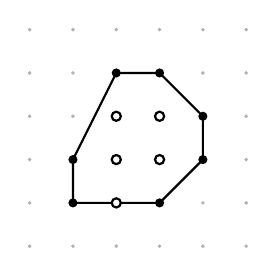
\begin{tikzpicture}[scale=0.55]
\foreach \x in {-2,...,3} \foreach \y in {-2,...,3} \fill[gray!60] (\x,\y) circle (1.3pt);
\draw[thick] (-1,-1)--(1,-1)--(2,0)--(2,1)--(1,2)--(0,2)--(-1,0)--cycle;
\foreach \p in {(-1,-1),(1,-1),(2,0),(2,1),(1,2),(0,2),(-1,0)} \fill \p circle (3pt);
\foreach \p in {(0,-1),(0,0),(0,1),(1,0),(1,1)} \draw[fill=white,thick] \p circle (3pt);
\end{tikzpicture}
\caption{The heptagon $P_2$: vertices black, non-vertex lattice points white.}
\label{fig:hept}
\vspace{-2ex}
\end{wrapfigure}
\paragraph{$n=1$ and $n=2$.} For $n=1$ take the segment $[0,6]$: two vertices
and five non-vertex lattice points $1,\dots,5$. For $n=2$ take the heptagon
$P_2$ with vertices
\[
(-1,-1),\ (1,-1),\ (2,0),\ (2,1),\ (1,2),\ (0,2),\ (-1,0),
\]
whose non-vertex lattice points are $(0,-1)$ on the boundary and
$(0,0),(0,1),(1,0),(1,1)$ in the interior (Figure~\ref{fig:hept}). A polygon with these numbers is also shown
in~\cite[Figure~1]{chz}.


\paragraph{$n=3$.} Let $P_3\subseteq\R^3$ be the convex hull of the $18$ points
\begin{gather*}
(-1,-1,1),\ (-1,0,0),\ (-1,0,1),\ (-1,1,0),\ (0,-1,0),\ (0,-1,1),\\
(0,0,-1),\ (0,1,-1),\ (0,1,1),\ (0,2,0),\ (1,-1,0),\ (1,0,-1),\\
(1,0,1),\ (1,1,-1),\ (1,1,1),\ (1,2,0),\ (2,0,0),\ (2,1,0).
\end{gather*}
All $18$ are vertices, and the other lattice points of $P_3$ are the five
points $(0,0,0)$, $(0,0,1)$, $(0,1,0)$, $(1,0,0)$, $(1,1,0)$; the point
$(0,0,1)$ lies on the boundary and the other four in the interior.

\paragraph{$n=4$.} It is convenient to work in the affine lattice
$L=\{x\in\Z^5:\ x_0+x_1+x_2+x_3+x_4=1\}$ with the unit vectors
$e_0,\dots,e_4$; deleting the last coordinate is an affine bijection from $L$
onto $\Z^4$ (its inverse appends $1-x_0-x_1-x_2-x_3$), and it maps lattice
polytopes in the hyperplane of $L$ to lattice polytopes in $\R^4$ with the same
vertices and lattice points. Let $P_4$ be the convex hull of the $37$ points
\begin{itemize}
\item $e_i+e_j-e_l$ for every pair $\{i,j\}$ and every $l\notin\{i,j\}$
($10\cdot3=30$ points);
\item $2e_1-e_0$ and $2e_0-e_i$ for $i=1,2,3,4$ ($5$ points);
\item $y=(1,1,1,-1,-1)$ and $2e_0-y=(1,-1,-1,1,1)$ ($2$ points).
\end{itemize}
All $37$ points are vertices, and the other lattice points of $P_4$ are exactly
$e_0,\dots,e_4$; for instance $e_i$ is the midpoint of $e_i+e_j-e_l$ and
$e_i+e_l-e_j$. Deleting the last coordinate maps this list exactly onto the
$37$ points of \texttt{FiniteGeometry.WitnessFour.vertices} and $e_0,\dots,e_4$ onto
$(1,0,0,0)$, $(0,1,0,0)$, $(0,0,1,0)$, $(0,0,0,1)$, $(0,0,0,0)$ (checked by
computation); Lean works with these coordinates in $\Z^4$.

\paragraph{The certificates.} For the polytopes of dimensions $2$, $3$, $4$ (and
the two polytopes $Q_\pm$ below), the Lean files check by kernel evaluation:
every listed vertex is the unique maximizer, among the listed points, of an
explicit integer linear function, so it is a vertex; every listed non-vertex
point is the midpoint of two listed vertices; all listed points lie in the box
$[-1,2]^d$; and every other lattice point of the box violates an explicit
integer inequality that holds on all listed points. Since the lattice points of
the hull lie in the box of the coordinate ranges, this determines the vertices
and all lattice points of the polytope.

\paragraph{Two empty polytopes inside $P_4$.} Let $Q_+$ and $Q_-$ be the convex
hulls of the following $16$ points each (in the coordinates of $L$):
\begin{align*}
Q_+:\ & e_0,\dots,e_4,\ 2e_0-y,\ e_0+e_2-e_1,\ e_0+e_2-e_3,\ e_0+e_3-e_1,\ e_0+e_4-e_1,\ e_0+e_4-e_2,\\
& e_0+e_4-e_3,\ e_1+e_2-e_3,\ e_1+e_4-e_2,\ e_1+e_4-e_3,\ e_3+e_4-e_2;\\
Q_-:\ & e_0,\dots,e_4,\ y,\ e_0+e_1-e_2,\ e_0+e_1-e_3,\ e_0+e_1-e_4,\ e_0+e_2-e_4,\ e_0+e_3-e_2,\\
& e_0+e_3-e_4,\ e_1+e_2-e_4,\ e_2+e_3-e_1,\ e_2+e_3-e_4,\ e_3+e_4-e_1 .
\end{align*}
Each is a lattice polytope whose $16$ lattice points are exactly its $16$
vertices, and $Q_\pm\subseteq P_4$. Their vertex sets meet exactly in
$e_0,\dots,e_4$, so no vertex of $P_4$ belongs to both.

\paragraph{The lift to $n=4+r$, $r\ge1$.} Let $U=\{0,1\}^r\setminus\{0\}$ and,
in $\R^4\times\R^r$ (with $\R^4$ carrying the coordinates of $\Z^4$),
\[
T=\conv\Bigl(\bigl(P_4\times\{0\}\bigr)\cup\bigl(Q_+\times U\bigr)\cup\bigl(Q_-\times(-U)\bigr)\Bigr).
\]
We show that the lattice points of $T$ that are not vertices are the five
points $(e_i,0)$, and that all other lattice points of $T$ are vertices; then
\[
|\vertx(T)|=37+2\cdot16\cdot(2^r-1)=2^{r+5}+5=2^{n+1}+5 .
\]
\begin{itemize}
\item \emph{The projection.} The projection of $T$ to $\R^r$ is
$B=\conv(U\cup-U)$. A point of $B$ has coordinates in $[-1,1]$, and no two of
its coordinates differ by more than~$1$; so the lattice points of $B$ are
$0$, $U$ and $-U$. Each $u\in U$ is the unique maximizer on $B$ of the linear
function with weight $+1$ on the coordinates where $u_i=1$ and $-1/(2r)$
elsewhere; similarly for $-U$.
\item \emph{The fibres over $\pm U$.} Since $u$ is exposed in $B$, the fibre of
$T$ over $u\in U$ is a face of $T$ and is the convex hull of the generators
over $u$, namely $Q_+$; its $16$ lattice points are vertices of $Q_+$ and hence
of $T$. The same holds
for $-U$ and $Q_-$.
\item \emph{The fibre over $0$.} It is $P_4$, because the first components of
all generators lie in $P_4$ (as $Q_\pm\subseteq P_4$). So its lattice points are
the $37+5$ lattice points of $P_4$, and the $(e_i,0)$ are still midpoints, so
not vertices.
\item \emph{The old vertices survive.} Let $p$ be a vertex of $P_4$ and write
$(p,0)$ as a convex combination of generators with positive weights. Since all
first components lie in $P_4$ and $p$ is a vertex of $P_4$, every generator used
has first component $p$. As $p$ lies in at most one of $Q_+$ and $Q_-$, all
second components lie in $\{0\}\cup U$ or all in $\{0\}\cup(-U)$; their positive
average is $0$, so all are $0$. Hence $(p,0)$ is a vertex of $T$.
\end{itemize}
As a check, our computation for $r=1$
found $69$ vertices and $74$ lattice points; one final reviewer also checked
$r=2$ ($133$ vertices).

\begin{proof}[Proof of Theorem~\ref{thm:main}]
By this section and Proposition~\ref{prop:transfer}(a), there is a
lattice polytope with $v(n)$ vertices and exactly five non-vertex lattice
points, so $g(\Z^n,5)\ge v(n)$ and $c(\Z^n,5)\ge v(n)$. By
Theorem~\ref{thm:poly} and Proposition~\ref{prop:transfer}(b) with $b=v(n)$,
$c(\Z^n,5)\le v(n)$ and $g(\Z^n,5)\le v(n)$.
\end{proof}

{\sloppy
\section{Formal verification}\label{sec:lean}

Theorem~\ref{thm:main} is formally verified in Lean~4 (version 4.34.1) with
Mathlib~\cite{mathlib} (commit \texttt{d13f23b7}), as the two statements
\texttt{TaskT.HellyFive.ExactHellyFive} (part~(i), the value of $c$) and
\texttt{TaskT.HellyFive.ExactVertexFive} (part~(ii), the value of $g$). The
$35$ files are in version~\repoversion{} of the repository~\cite{repo},
directory \texttt{lean/Research/TaskT/HellyFive/}: the $31$ modules in the
import closure of \texttt{Check.lean} (including it), and four auxiliary audit
modules (\texttt{BridgeAudit}, \texttt{FiniteAudit},
\texttt{FiniteHellyLower}, \texttt{UpperTransferAudit}) that print axioms and
restate two intermediate lower bounds ($18$ and $37$); nothing in the proof
depends on them. Records of the freezing and of the checks are in the folder
\texttt{certificates/quantitative-helly-five}.

\paragraph{The statements.} The statement file \texttt{Challenge.lean}, in
ASCII transliteration (the \texttt{import Mathlib} line, the
\texttt{namespace TaskT.HellyFive} and \texttt{end} lines and three docstrings
are omitted; the file uses Unicode: \texttt{Nat}, \texttt{Int}, \texttt{Real}
and \texttt{ENat} stand for $\mathbb N$, $\Z$, $\R$ and $\mathbb N_\infty$,
\texttt{->} for $\to$, \texttt{forall}, \texttt{exists}, \texttt{in},
\texttt{notin}, \texttt{/\char`\\} and \texttt{<=} for $\forall$, $\exists$,
$\in$, $\notin$, $\wedge$ and $\le$):
{\footnotesize
\begin{verbatim}
abbrev Space (n : Nat) := Fin n -> Real
abbrev Grid (n : Nat) := Fin n -> Int
def embed {n : Nat} (x : Grid n) : Space n := fun i => x i
def commonGrid {n m : Nat} (C : Fin m -> Set (Space n)) (s : Finset (Fin m)) :
    Set (Grid n) :=
  {z | forall i in s, embed z in C i}
def PreservesFive (n t : Nat) : Prop :=
  forall (m : Nat), 0 < m -> forall C : Fin m -> Set (Space n),
    (forall i, Convex Real (C i)) -> (commonGrid C Finset.univ).encard = 5 ->
    exists s : Finset (Fin m), s.card <= t /\ (commonGrid C s).encard = 5
def attainableCounts (n : Nat) : Set Nat :=
  {t | exists V : Finset (Grid n),
    let P := convexHull Real (embed '' (V : Set (Grid n)))
    (P.extremePoints Real).encard = (t : ENat) /\
      ({z : Grid n | embed z in P /\ embed z notin P.extremePoints Real} :
        Set (Grid n)).encard = 5}
def value (n : Nat) : Nat :=
  if n = 1 then 2 else if n = 2 then 7 else if n = 3 then 18 else 2 ^ (n + 1) + 5
def ExactHellyFive : Prop :=
  forall n : Nat, 0 < n -> IsLeast {t : Nat | PreservesFive n t} (value n)
def ExactVertexFive : Prop :=
  forall n : Nat, 0 < n -> IsGreatest (attainableCounts n) (value n)
\end{verbatim}}
\noindent The two line breaks inside \texttt{commonGrid} and
\texttt{attainableCounts} are ours. Here \texttt{Grid n} is $\Z^n$ and
\texttt{embed} its inclusion in $\R^n$. \texttt{commonGrid C s} is the set of
lattice points common to the sets $C_i$, $i\in s$ (all of $\Z^n$ for the empty
$s$). \texttt{PreservesFive n t} says that $t$ is admissible in
Definition~\ref{def:c} for $S=\Z^n$ and $k=5$: for every $m\ge1$ and every
family of $m$ convex sets (repetitions allowed, not necessarily closed or
bounded) with exactly five common lattice points, some subfamily of at most $t$
sets has exactly five common lattice points (then necessarily the same five).
\texttt{encard} is the cardinality in $\mathbb N\cup\{\infty\}$, so an infinite
set never counts as five. \texttt{attainableCounts n} is the set of numbers of
vertices (extreme points) of lattice polytopes in $\R^n$, of any dimension and
with redundant generators allowed, that have exactly five non-vertex lattice
points, boundary points included. \texttt{IsLeast A v} means $v\in A$ and $v\le a$
for all $a\in A$, and \texttt{IsGreatest} is the dual; so
\texttt{ExactHellyFive} says $c(\Z^n,5)=v(n)$ and \texttt{ExactVertexFive} says
$g(\Z^n,5)=v(n)$, for every $n\ge1$ (the case $n=0$ of \texttt{value} lies
outside the quantifier). The final reviewers restated both statements with all
definitions written out inline and proved them from the \texttt{Proof}
theorems, so no shadowing or redefinition can weaken them.

\paragraph{Review and freezing.} \texttt{Challenge.lean} was compared with the
source by Codex, compiled with no diagnostics (01:10:41--01:11:05~UTC on
21 November 2026), reviewed by a Codex agent that had written neither the
statement nor the proofs (approval at 01:11:14~UTC), and frozen by recording
its SHA-256 hash (\texttt{faf32ea5\ldots}) at 01:11:55~UTC. The compilation
receipts record no compilation of a proof file before the freeze (the first
is at 01:12:45~UTC), and the file was not changed afterwards.

\paragraph{The proofs.} The check file \texttt{Check.lean} contains, apart
from \texttt{import} and \texttt{namespace} lines and a line
\texttt{export TaskT.HellyFive (ExactHellyFive ExactVertexFive)} inside
\texttt{namespace Challenge}, exactly
{\footnotesize
\begin{verbatim}
theorem check_ExactHellyFive : Challenge.ExactHellyFive := Proof.ExactHellyFive
theorem check_ExactVertexFive : Challenge.ExactVertexFive := Proof.ExactVertexFive
\end{verbatim}}
\noindent together with four \texttt{\#print axioms} commands; the
\texttt{export} makes \texttt{Challenge.ExactHellyFive} the frozen constant
itself. Table~\ref{tab:lean} lists the Lean counterparts of the steps (names
relative to the namespace \texttt{TaskT.HellyFive}; file names in parentheses,
without \texttt{.lean}).

\begin{table}[!htbp]
\centering\footnotesize
\renewcommand{\arraystretch}{1.05}
\begin{tabular}{@{}>{\raggedright\arraybackslash}p{0.30\textwidth}>{\raggedright\arraybackslash}p{0.66\textwidth}@{}}
\hline
Step of the written proof & Lean (file) \\
\hline
Proposition~\ref{prop:transfer}(a) &
\texttt{attainableCount\_le\_preservingBound} (\texttt{LowerTransfer}) \\
Proposition~\ref{prop:transfer}(b), for $c$ &
\texttt{preservesFive\_of\_polyBound} (\texttt{UpperTransfer});
\texttt{UpperTransfer.extend\_closed} (\texttt{UpperTransferGeometry});
\texttt{UpperTransfer.maximalContacts} (\texttt{UpperTransferMaximal});
\texttt{UpperTransfer.PolyBound}, \texttt{UpperTransfer.countContacts}
(\texttt{UpperTransferCount}) \\
Lemma~\ref{lem:mid} & \texttt{gridMid\_mem\_nonvertices} (\texttt{Midpoints}) \\
Lemma~\ref{lem:triple}, Proposition~\ref{prop:charge} &
\texttt{UpperFive.recover\_triangle}, \texttt{UpperFive.charge},
\texttt{UpperFive.all\_dimensional\_bound}
(\texttt{UpperCharge}) \\
Theorem~\ref{thm:poly}, $n\ge4$ (from polytopes to finite sets) &
\texttt{UpperFive.card\_decomposition}, \texttt{UpperFive.apply\_bound},
\texttt{UpperFive.high\_upper} (\texttt{UpperGeom}) \\
Theorem~\ref{thm:poly}, $n=3$ (capacities, padding $X$) &
\texttt{UpperFive.capacity}, \texttt{UpperFive.card\_le\_capacity},
\texttt{UpperFive.indexed\_cover} (\texttt{UpperWeights});
\texttt{UpperFive.sorted\_table} (\texttt{UpperThreeTable});
\texttt{UpperFive.three\_capacity}, \texttt{UpperFive.three\_upper},
\texttt{UpperFive.upper\_of\_poly} (\texttt{UpperThree}) \\
Theorem~\ref{thm:poly}, $n=2$ &
\texttt{PlanarData.table}, \texttt{PlanarData.classify} (\texttt{PlanarTable});
\texttt{PlanarObstruction.balanced\_four},
\texttt{PlanarObstruction.cross\_of\_balanced} (\texttt{PlanarObstructionCross});
\texttt{PlanarObstruction.obstruction} (\texttt{PlanarObstruction});
\texttt{PlanarUpper.count\_five}, \texttt{PlanarUpper.upper} (\texttt{PlanarUpper}) \\
Theorem~\ref{thm:poly}, $n=1$, and the segment &
\texttt{DimensionOne.extreme\_card\_le}, \texttt{DimensionOne.attainable}
(\texttt{DimensionOne}) \\
Theorem~\ref{thm:poly}, all $n$ & \texttt{Proof.poly\_bound} (\texttt{Proof}) \\
Certificates of vertices and lattice points &
\texttt{FiniteGeometry.extremal\_of\_unique\_row},
\texttt{FiniteGeometry.strictly\_separated}, \texttt{FiniteGeometry.grid\_box},
\texttt{FiniteGeometry.cube\_repr}, \texttt{FiniteGeometry.realization}
(\texttt{FiniteGeometry}) \\
$P_2$, $P_3$, $P_4$ &
\texttt{FiniteGeometry.WitnessTwo.attainable},
\texttt{FiniteGeometry.WitnessThree.attainable},
\texttt{FiniteGeometry.WitnessFour.attainable} (\texttt{WitnessTwo},
\texttt{WitnessThree}, \texttt{WitnessFour}) \\
$Q_\pm$ &
\texttt{FiniteGeometry.CorePositive.geometry},
\texttt{FiniteGeometry.CoreNegative.geometry} (\texttt{CorePositive},
\texttt{CoreNegative}); \texttt{FiniteGeometry.positive\_subset},
\texttt{FiniteGeometry.negative\_subset},
\texttt{FiniteGeometry.disjoint\_at\_old\_extreme} (\texttt{FiniteKernels}) \\
The lift &
\texttt{FiberProjection.body\_grid\_iff}, \texttt{FiberProjection.positive\_fiber},
\texttt{FiberProjection.zero\_fiber}, \texttt{FiberProjection.central\_extreme\_iff},
\texttt{FiberProjection.nonvertex\_grid\_iff} (\texttt{FiberProjection});
\texttt{Lift.seed\_card}, \texttt{Lift.extreme\_lifted\_eq} (\texttt{LiftLayers});
\texttt{Lift.joined\_nonvertex}, \texttt{Lift.attainable\_ge\_four}
(\texttt{LiftAttainable}) \\
Theorem~\ref{thm:main} &
\texttt{Proof.attained}, \texttt{Proof.ExactHellyFive},
\texttt{Proof.ExactVertexFive} (\texttt{Proof}) \\
\hline
\end{tabular}
\caption{Lean counterparts of the steps of the proof.}
\label{tab:lean}
\end{table}

\noindent The Lean proofs do not assume any result of~\cite{agm}
or~\cite{chz}: the transfer between convex sets and polytopes, the planar value
and the lower bounds are proved again. The axioms of
\texttt{Proof.ExactHellyFive}, \texttt{Proof.ExactVertexFive},
\texttt{check\_ExactHellyFive} and \texttt{check\_ExactVertexFive} are exactly
\texttt{propext}, \texttt{Classical.choice} and \texttt{Quot.sound}. No file
uses \texttt{sorry}, \texttt{native\_\allowbreak decide},
\texttt{bv\_\allowbreak decide} or an \texttt{axiom} declaration; all uses of
\texttt{decide}, including the two classification tables and the certificate
checks, are checked by the kernel. The only options set are
\texttt{maxHeartbeats 0} and \texttt{maxRecDepth}, in the data, table and
polytope files.

\paragraph{Checks.} The $31$ modules in the import closure of
\texttt{Check.lean} were compiled module by module in two new empty directories
on the author's Mac, with the pinned toolchain and with warnings treated as
errors, on 21 November 2026 (01:36:18--02:13:44~UTC, the second directory from
01:58:30~UTC); each directory also ran one build of the whole package, and
every module was replayed with \texttt{leanchecker}. All $126$ commands ($63$
per directory) ended with exit code~$0$, the \texttt{leanchecker} runs printed
nothing, and the two directories produced identical \texttt{.olean} files. The
two table modules used up to $14.01$~GB of memory per command. The final
reviewers (see the next section) compiled all $35$ files again with plain
\texttt{lean} in new directories of their own, together with short audit files
of their own, and replayed every module with \texttt{leanchecker} (one reviewer between
03:22 and 03:34~UTC; the other built its heavy modules between 04:18 and
04:28~UTC); all $36$ modules of each rebuild compiled with exit code~$0$ and no
warnings, and all \texttt{leanchecker} runs ended with exit code~$0$ and empty
output. Mathlib and its dependencies were taken from a shared prebuilt cache
at the pinned commits and were not rechecked; the \texttt{leanchecker} replays
cover the project modules. In the repository the files have module names under
\texttt{Research.TaskT.HellyFive} and differ from the checked files only in
their \texttt{import} lines (\texttt{Challenge.lean}, which imports only
Mathlib, is unchanged).
These versions were compiled and replayed with \texttt{leanchecker} again, module by module, in two new empty directories on the author's Mac (22 November 2026, 21:08--21:33~UTC), with no warnings and identical \texttt{.olean} files and the same axiom lists.
In the whole-project rebuild of version~\repoversion{} of the repository (on the author's Windows computer, in one pass from 22 to 23 November 2026), these files were compiled and replayed with \texttt{leanchecker} again together with the rest of the project; no module needed a second attempt (details in the repository). The formalization has not been checked with comparator or with
an independent kernel.

\par}

\section*{How this paper was produced}
This work was carried out from 21 to 23 November 2026 (UTC) in a workflow
directed by the author, using OpenAI Codex with the model GPT-6.2-Astra
(reasoning level ultra) and Anthropic Claude Code with the model Claude
Opus~5.5. The author asked for a new round of search for major open problems, and
Claude Code passed this request to Codex at 01:00~UTC on 21 November. In that
search Codex screened $72$ problems not screened in earlier rounds and prepared
notes on eight of them, this one among them. According to the file times, by
01:05~UTC a Codex agent had found the four-dimensional polytope and the upper
bound $2^{n+1}+5$, and soon afterwards the polytopes for $n=3$ and $n\ge5$; the
written proof for all dimensions was read by another Codex agent (same model)
that had not taken part in it, which approved it at 01:09~UTC, and two
passages of the manuscript were then revised (the quotation of the
recursion~\eqref{eq:rec} and the labelling of a superseded paragraph). As the task description
allowed for a complete written proof approved in this way, Codex then wrote
the statement file, had it reviewed and froze it as described in Section~\ref{sec:lean}
and began the Lean proof. The search ended at 01:22~UTC with this problem
ranked first. Under the same clause, which lets such a result go on to the
freeze and the Lean proof without waiting for the author, Claude Code resumed
the Codex session at 01:22~UTC (the time stamp of its instruction in the
session log) to complete the formalization. According to the file timestamps and the compilation receipts, the
proof files were created after the freeze and compiled during development
between 01:12 and 01:35~UTC. The formal upper bound does not follow the written
case analysis (Remark~\ref{rem:written}): it counts all lattice points of the
polytope and uses the two tables and the planar argument of
Section~\ref{sec:upper}. A Codex agent that had not written the proofs read
the source files against the definitions (01:35~UTC) before the checks
described in Section~\ref{sec:lean}.

The final reviews were done by two Claude Code agents (model Claude Opus~5.5)
that had written none of the files, from 03:20~UTC; neither read the other's
report. Each reviewer read the sources itself, compared the statement file with
them, read the written proofs and the proof files, checked the receipts of the
checks, recomputed the polytopes and the capacity tables with its own
programs, and rebuilt the formalization as described above; one also
enumerated the $33{,}041$ convex lattice polygons in $[0,4]^2$ (recovering
$g(\Z^2,k)$ of~\cite{agm} for $k\le8$), the other checked the lift for $n=5,6$.
The decisions were APPROVE\_FORMAL and APPROVE\_WITH\_CHANGES, with no
blocking or major remarks; the minor remarks ($6$ and $7$, two of them
optional) concern the written account and the attribution, and are taken into
account here (among them the route of the formal upper bound, the attributions
to~\cite{agm,chz}, the scope of Definition~\ref{def:c}, Open question~3
of~\cite{agm}, the auxiliary modules, the coordinates of $P_4$, and the reading
of~\cite{hn}, whose full text the reviewer could not access). Claude Code (Claude Opus~5.5) checked the
sources, recomputed in Python the vertices and lattice points of $P_2$, $P_3$,
$P_4$, $Q_\pm$ and of the lift for $n=5$, the coordinates of $P_4$ in $L$ and in
$\Z^4$, and the distributions of the capacity sums, and wrote this text from
Codex's manuscripts and the Lean files; the account of the formal route in
Section~\ref{sec:upper}, including the planar argument, was written from the
Lean files and was not part of the documents read by the final reviewers. An independent Claude Code agent (model Claude Opus~5.5) that had written none of the files reviewed this paper, and two others reviewed the release; their corrections were applied. Throughout,
``we'' refers to this workflow; the reading and searching described in the
paper were done by the agents. Codex agents searched for prior work in the
search for problems, including an independent search by an agent that had not
worked on the proof (completed at 01:17~UTC on 21 November); the second final
reviewer searched again on 21 November (arXiv queries, the OpenAlex and
Semantic Scholar lists of works citing~\cite{abdl,agm,chz}, zbMATH Open,
Crossref, the OEIS, GitHub and general web searches); and on 22 November 2026 (19:22~UTC) an
independent Claude Code agent (Claude Opus~5.5) read the full text
of~\cite{hn}, from a licensed copy downloaded by the author, and found in it no exact value of $c$ or $g$ and no counterpart of our
constructions.
Up to 22~November 2026 these searches found no earlier determination of
$c(\Z^n,5)$ or $g(\Z^n,5)$ for any $n\ge3$, of the value $18$, or of the
formula $2^{n+1}+5$ (details in the repository). On 23~November 2026 (11:10--11:28~UTC) Claude Code searched again (the arXiv, the OpenAlex and Semantic Scholar lists of works citing the main sources, Zenodo, DataCite, GitHub and repositories of AI-assisted mathematics) and found no new related work. This
reports the coverage of the searches, not a guarantee that they were complete.
The author is not a professional mathematician. The author has read this paper and, using a side-by-side table, compared its Lean statements with Theorem~\ref{thm:main}. No human
mathematician has read the proofs or reviewed this paper. The correctness of
Theorem~\ref{thm:main} rests on the Lean proofs and on the agreement of the
Lean statements with the definitions of~\cite{agm}; the written proofs are given
for the reader. AI systems are not authors of this paper; the author takes full
responsibility for its content.

\medskip
\noindent Thanks are due to Gennadiy Averkov, Bernardo Gonz\'alez Merino,
Matthias Henze, Ingo Paschke, Matthias Schymura and Stefan Weltge for the
framework and the values on which this work rests, and to Stephen R. Chestnut,
Robert Hildebrand and Rico Zenklusen for the planar value and the parity
method.

{\small
\begin{thebibliography}{9}
\setlength{\itemsep}{1pt}
\bibitem{abdl} I.~Aliev, R.~Bassett, J.~A. De~Loera and Q.~Louveaux, A
quantitative Doignon--Bell--Scarf theorem, \emph{Combinatorica} 37 (2017),
no.~3, 313--332, \url{https://doi.org/10.1007/s00493-015-3266-9};
arXiv:1405.2480v3 (2015).
\bibitem{agm} G.~Averkov, B.~Gonz\'alez Merino, I.~Paschke, M.~Schymura and
S.~Weltge, Tight bounds on discrete quantitative Helly numbers, \emph{Adv.
Appl. Math.} 89 (2017), 76--101,
\url{https://doi.org/10.1016/j.aam.2017.04.003}. Preprint version:
G.~Averkov, B.~Gonz\'alez Merino, M.~Henze, I.~Paschke and S.~Weltge,
arXiv:1602.07839v1 (2016).
\bibitem{chz} S.~R. Chestnut, R.~Hildebrand and R.~Zenklusen, Sublinear bounds
for a quantitative Doignon--Bell--Scarf theorem, \emph{SIAM J. Discrete Math.}
32 (2018), no.~1, 352--371, \url{https://doi.org/10.1137/16M1100095};
arXiv:1512.07126v2 (2017).
\bibitem{repo} H.~Dong, \emph{ai4math-results}, repository,
\url{https://github.com/Horace-Maxwell/ai4math-results}, version~\repoversion{}
(2026); archived at Zenodo under the concept DOI
\url{https://doi.org/10.5281/zenodo.22970254}.
\bibitem{doi} J.-P. Doignon, Convexity in cristallographical lattices,
\emph{J. Geom.} 3 (1973), no.~1, 71--85,
\url{https://doi.org/10.1007/BF01949705}.
\bibitem{hn} M.~Huicochea and B.~Navarro, Midpoints of vertex pairs of convex
polytopes, \emph{SIAM J. Discrete Math.} 39 (2025), no.~3, 1806--1825,
\url{https://doi.org/10.1137/24M1714496}.
\bibitem{mathlib}
The mathlib Community, The Lean mathematical library, in \emph{Proc.\ 9th ACM
SIGPLAN Int.\ Conf.\ Certified Programs and Proofs} (CPP '20), ACM, 2020,
367--381, \url{https://doi.org/10.1145/3372885.3373824}.
\end{thebibliography}}
\end{document}
